\chapter{Podaci}
\label{chap:podaci}

Orthobalancer radi sa primarnim proteinskim strukturama --- sekvencama
reziduuma, odnosno aminokiselina. Za zapis sekvenci koristi se standardizirani
FASTA format. Orthobalancer za svoj rad koristi dvije
NCBI-jevih\footnote{National Center for Biotechnology Information} baza
podataka od kojih jedna sadrži sekvence formatirane u FASTA format, a druga
taksonomsko stablo živog svijeta.


\section{FASTA format}


\section{Neredundantna baza}


\section{Taksonomsko stablo živog svijeta}


\section{Ulaz}

Aplikacija kao ulaz prima nekolicinu paralognih proteina u FASTA formatu. Ako
korisnik posjeduje samo sekvencu proteina, može ju zadati bez FASTA zaglavlja,
no u tome je slučaju dužan dati ime unesenoj sekvenci. Nužno je imati ime za svaki
ulazni paralog te je nužno da da su sva međusobno jedinstvena.

Dodatno, korisnik može specificirati čvorove taksonomskog stabla za čija
podstabla smatra da sadrže zamjenjive vrste. Ponuđen je i osnovni skup
zamjenskih čvorova za koje se vjeruje da bi mogli biti od koristi korisniku.


\section{Izlaz}

Web aplikacija za završetak izvođenja prikazuje tablicu balansiranih vrsta.
Stupci tablice su imenovani po paralozima s ulaza. Retci su grupirani u
zamjenske čvorove. Svaki redak predstavlja jedan balansirani skup vrsta. U
stupcu pod pojedinim paralogom nalazi se ortologna vrsta, a lijevo od svih vrsta
je zapisan čvor na kojem su vrste tog retka balansirane. Primjer tablice se može
vidjeti naslici \ref{fig:tablica}.

\begin{figure}[h!]
\centering
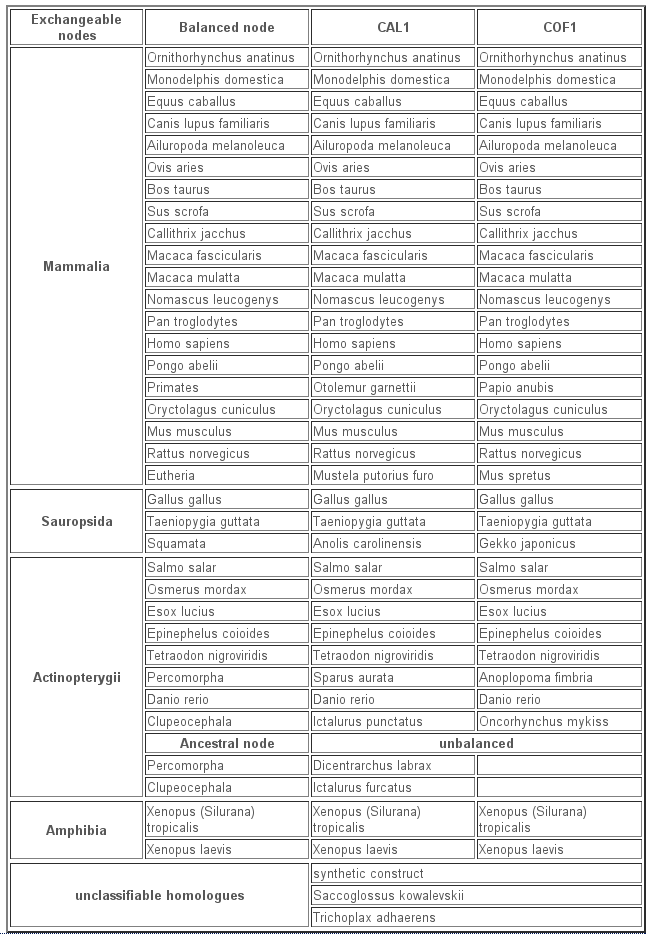
\includegraphics[width=4.75in]{figures/tablica.png}
\caption{Izlazna tablica sa web stranice Orthobanalcera}
\label{fig:tablica}
\end{figure}

Također, završna stranica sadrži poveznice za preuzimanje generiranih datoteka
tijekom izvođenja. Datoteke su opisane u nastavku.
